\documentclass[twocolumn,superscriptaddress,aps]{revtex4-1}

\usepackage[utf8]{inputenc}

\usepackage{amsfonts}
\usepackage{amssymb}
\usepackage{amsmath}
\usepackage{amsthm}

\usepackage{bbold}
\usepackage{bm}
\usepackage{graphicx}
\usepackage{color}
\usepackage{hyperref}

%\usepackage[export]{adjustbox}
\DeclareMathOperator*{\argmin}{arg\,min}

\begin{document}


% ==============================================================================

\title{\Large{INFO8004: A review of the Information Bottleneck in Deep Learning}}
\vspace{1cm}
\author{\small{\bf Eduardo V. Gandara}}
\affiliation{\texttt{e.varas@student.uliege.be} (\texttt{s184314})}
\author{\small{\bf Aurélien Werenne}}
\affiliation{\texttt{awerenne@student.uliege.be} (\texttt{s110995})}

\maketitle

% ==============================================================================

\section*{Abstract}

Deep Neural Networks are used in many applications nowadays, from image classification to speech recognition, achieving human-level performance. Paradoxically, the success of Deep Learning (DL) is far from being fully understood. Why are deep learning models able to generalize? Why is the performance increased when stacking more layers? An attempt to answer those questions is made with the Information Bottleneck theory. The objective of this review paper is i) to present the fascinating results obtained by applying the Information Bottleneck to DL ii) to discuss the limitations of the theory iii) explore potential applications. 


\section{Introduction}

For the course INFO8004 the assignment of our group was to analyse and summarize the Information Bottleneck (IB) and how it is used to interpret Deep Neural Networks (DNN) \citep{Tishby2, Tishby3}. In Section 2 of this paper the necessary background is presented to understand the Information Bottleneck. Section 3 then starts by presenting how the IB is applied to Deep Learning. Next, we explain the main results of the experiments performed by the authors. Lastly, the limitations and possible further applications that could be developed are discussed.


\section{Background}\label{sec:background}

\noindent \textbf{Mutual Information} \\[0.15cm]
\indent Let $X \in \mathcal{X}$ and $Y \in \mathcal{Y}$ be two random variables with a joint distribution $p(X,Y)$. The concept of Mutual Information (MI) is defined as
\begin{equation}
I(X;Y) = \mathbb{E} \left[log\left(\frac{p(X,Y)}{p(X)p(Y)} \right)\right]
\label{eq:mutual-info}
\end{equation}
For most distributions (except exponential distributions) direct MI computation is intractable. One common estimation technique is to discretize continuous variables by binning. The expectation expressed in (\ref{eq:mutual-info}) can then be approximated with sampling techniques. It is worth noticing that this binning process introduces some noise.\\

\noindent \textbf{Minimal Sufficient Statistics} \\[0.15cm]
\indent A \textit{sufficient statistic} is defined as the quantity of relevant information on the targets $Y$ contained in the observations $X$. More specifically, a probabilistic function $S(X)$ is a sufficient statistic for $Y$ if and only if
\begin{equation}
I(S(X);Y) = I(X;Y)
\label{eq:suff-stat}
\end{equation}
Furthermore, a \textit{minimal sufficient statistic} $T(X)$ is the optimal representation containing all the available information about $Y$, while being the best possible compression of $X$:

\begin{equation}
T(X) = \argmin_{S(X) \, : \, I(S(X);Y) = I(X;Y)} I(S(X);X)
\label{eq:min-suff-stat}
\end{equation}

\noindent \textbf{Information Bottleneck} \\[0.15cm]
\indent Solving the optimization problem (\ref{eq:min-suff-stat}) is in most practical problems (highly dimensional input space) difficult to compute. Inspired from the Rate-Distortion theory of Shannon, Tishby presented the IB method \citep{Tishby1} in order to turn this optimization problem solvable. Using the Lagrange relaxation, Equation (\ref{eq:min-suff-stat}) is solved like

\begin{equation}
\min_{p(t|x)} I(T;X) - \beta I(T;Y)
\label{eq:lagrange}
\end{equation}
with $\beta$ the Lagrange multiplier controlling the trade-off between the amount of information about $Y$ being compressed/preserved .

\section{Information Bottleneck and Deep Learning}

Let $X \in \mathcal{X}$ be the inputs and $Y \in \mathcal{Y}$ the ground-truth labels, the authors model the DNN as a Markov Chain where each hidden layer $i$ is represented as  a single random variable $T_i$. Thereupon, they proved experimentally that the hidden layers $T_i$ approach the IB optimal solution for different values of $\beta$ (see Figure 1).\\

\begin{figure}[!htb]
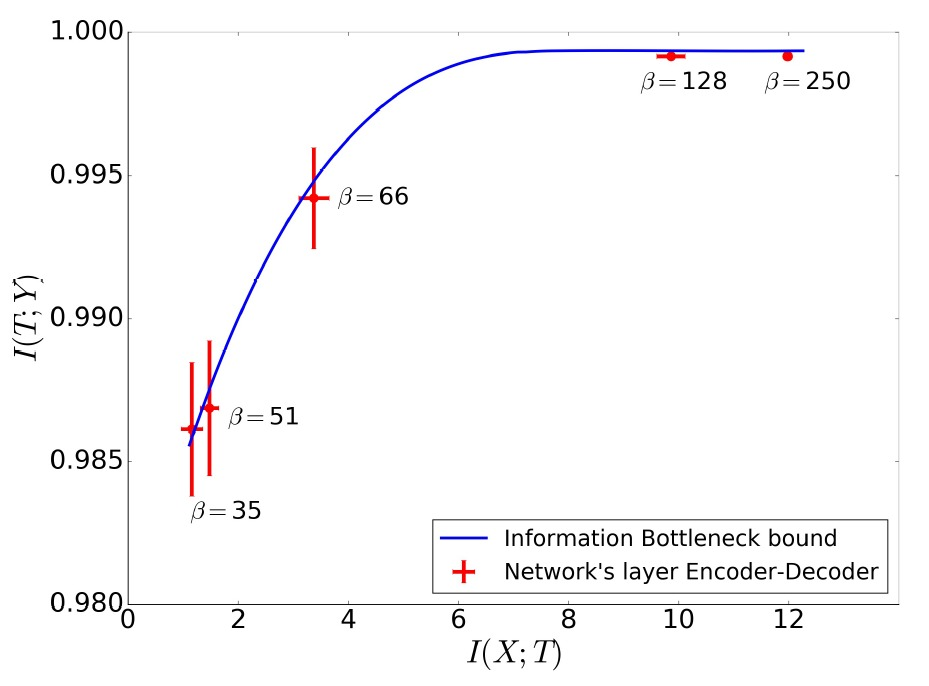
\includegraphics[width=\linewidth, height=\textheight, keepaspectratio]{figs/ib-curve.jpeg}
\label{fig:ib-curve}
\caption{The DNN layers converge to fixed-points of the IB equations. The error bars represent standard error measures with N=50. In each line there are 5 points for the different layers. For each point, $\beta$ is the optimal value that was found for the corresponding layer}
\end{figure}

\noindent \textbf{Information Plane} \\[0.15cm]
\indent One of the main contributions is the study of the learning process of neural networks in the information plane, introduced in \citep{Tishby2}. Their experiments using the information plane showed how mutual informations $I(T;X)$ and $I(T;Y)$ evolve during the optimization process (see figure and link to video in the original paper). Initially, it can be seen that the deeper layers fail to preserve the information about the input since the layers are randomly initialized. Moreover, Tishby et al. distinguish two phases observed visually. In the first phase of the learning process, the model fits to the data in order to improve its predictions. More interestingly, in the second much slower phase, mutual informations in the information plane move to the upper left corner, in other words, layers lose information about their input while slightly increasing information about the labels. Authors call this phase is the \textit{compression} or \textit{diffusion} phase. They claim that the compression part of the training is responsible for reducing generalization error.\\

\noindent \textbf{Stochastic Gradient Descent} \\[0.15cm]
\indent In our opinion, the most interesting part of the paper is the explanation of how neural networks achieve compression. Figure 2 displays the mean and variance of the gradients per layer. Notice that the two previously mentioned phases can be observed. For the first 300 epochs, the gradients have a high norm and very small deviations, then the variance grows larger until becoming more important than the mean. While the network is fitting the data, the loss is decreasing rapidly. As expected, this corresponds to large gradients with low variance. On the contrary, the compression phase has noisy gradients (i.e. high variance). The authors explain that Stochastic Gradient Descent with a noisy gradient is equivalent to a Random Walk in the parameter space of the loss function. As a consequence, random noise is added to the weights, leading to an increase in the entropy of layers $T_i$ with respect to the inputs. It is worth noticing that this occurs while keeping the training error stable.  The conditional entropy $H(X|T_i)$ being increased will cause a decrease of the mutual information $I(X;T_i)$, since the input entropy $H(X)$ remains unchanged.\\

\begin{figure}[!htb]
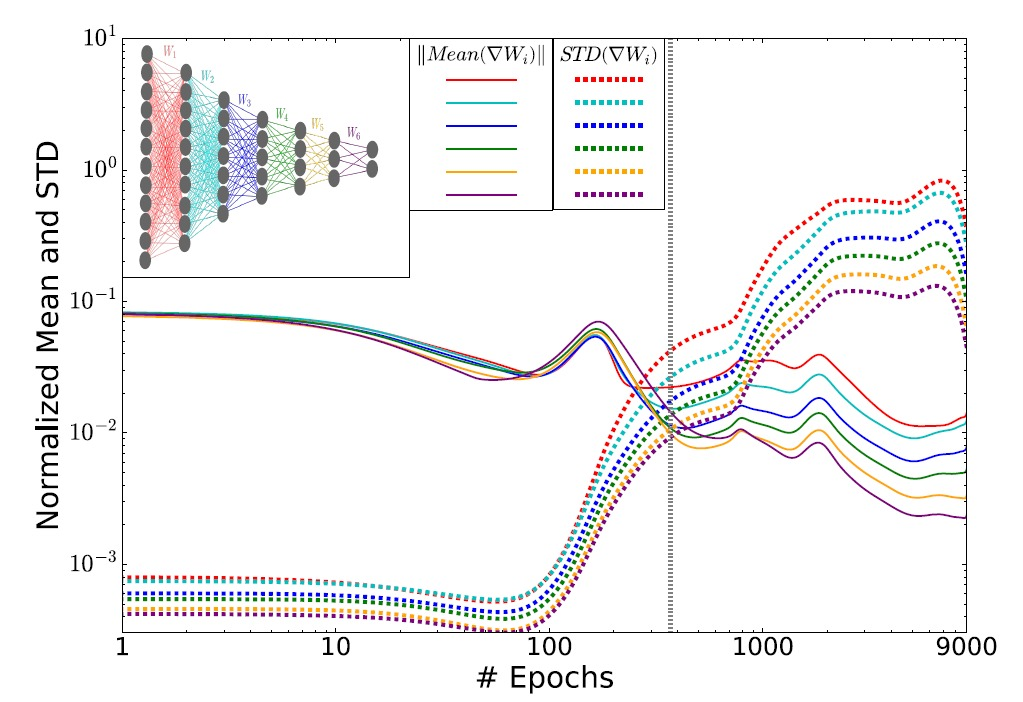
\includegraphics[width=\linewidth, height=\textheight, keepaspectratio]{figs/gradients.jpeg}
\label{fig:sgd}
\caption{The layers Stochastic Gradients distributions during the optimization process. The norm of the means and standard deviations of the weights gradients for each layer, as function of the number of training epochs (in log-log scale). }
\end{figure}


\noindent \textbf{Overfitting and Hidden Layers} \\[0.15cm]
\indent This new insight helps us better understand two well-known phenomena in deep learning: \textit{overfitting} and \textit{deeper models generalize faster}. \\
\indent \textit{Overfitting} can be interpreted in the information plane (see Figure 3). We observe that overfitting occurs mostly in the compression phase, where it seems that the representation in the layers is simplified too much. \\

\indent The computational benefit of deeper NN is according to the authors due to the fact that adding more hidden layers makes the compression go faster, i.e. generalizing faster. Indeed using the Focker-Plank equation \cite{fokker}, the quantity of entropy increase due to SGD follows the relationship
\begin{equation}
\Delta H \propto log(D\tau)
\label{eq:propto}
\end{equation}
with $D$ the diffusion constant and $\tau$ the number of epochs. Thus, the number of epoch needed to make a compression $\Delta I_X$ grows exponentially as $\text{exp}(\Delta I_X / D)$. If the compression task is shared among K hidden layers, each layer compresses $\Delta I^k_X$, where $\Delta I_X = \sum_k \Delta I^k_X$. Thereupon, the time needed for these K layers to achieve the compression, $\Delta I_X$, is $\sum_k \text{exp}(\Delta I^k_X/D)$. Since the exponential of a sum grows larger than the sum of an exponential, the authors deduce that compression is achieved faster in deeper networks.

\begin{figure*}[!htb]
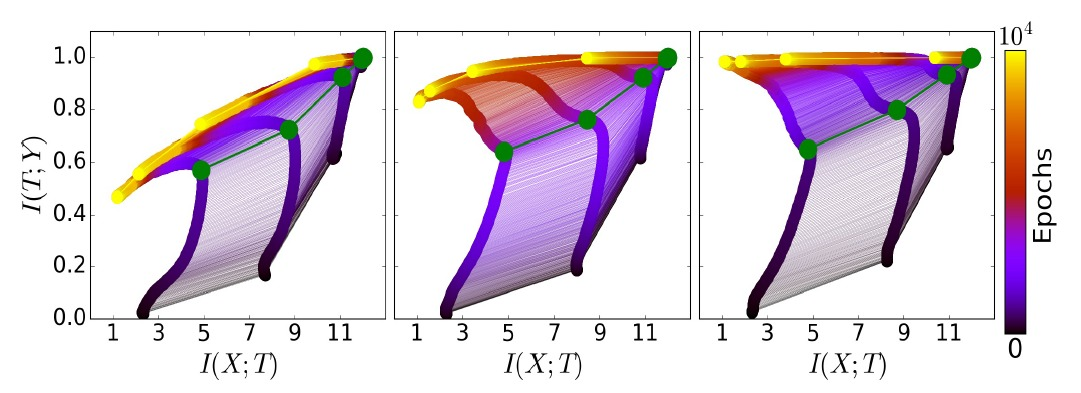
\includegraphics[width=\textwidth, height=\textheight, keepaspectratio]{figs/overfitting.jpeg}
\label{fig:overfitting}
\caption{The evolution of the layers with the training epochs in the information plane, for different training samples. On the left - 5\% of the data, middle - 45\% of the data, and right - 85\% of
the data. The colors indicate the number of training epochs with Stochastic Gradient Descent from 0 to 10000. The network architecture was fully connected layers, with widths:
input=12-10-8-6-4-2-1=output. The examples were generated by the spherical symmetric
rule described in the text. }
\end{figure*}

\section{Discussion}

A major drawback of the paper is that experiments where performed on a simple DNN with saturating activation functions. Saxe et al.\citep{saxe} showed that when using the very common ReLU function, the DNN yields no clear sign of compression. However Tishby claims the experiments of Saxe et al.\citep{saxe} are invalid because their methodology for estimating MI is not robust. This was indeed confirmed recently by Chelombiev et al.\cite{MI1}, they justified that a DNN using non-saturating functions, results in unbounded hidden activity. The level of noise brought by the binning process (see Section \ref{sec:background}) during the estimation becomes not consistent. To counter this undesired effect, Chelombiev et al.\cite{MI1} developed an adaptive estimator. Their findings showed in the information plane the fast fitting then slow compression pattern, even for a ReLU function.\\
\indent Another limitation of the paper is that it would have been easy to verify partially the conclusions on consequent datasets like ImageNet\cite{imagenet}. Indeed a common trick is to stop the training process once the validation error oscillates around its lowest point. The authors could have continued training for a long time and verify if the model does indeed generalize better, for example using adversarial examples.\\
\indent An important issue preventing the IB to be easily integrated in a DL setting is that mutual information estimation is computationally expensive in real-world machine learning problems. Possible solutions involve developing faster estimators \citep{MI1, MI2} or as suggested by Tishby in one of his talks, use the order of magnitude of the proportion between mean and variance of the gradients as a proxy for MI estimation. \\
\indent In \citep{vib} a very interesting relationship between Variational Auto-encoders (VAE) \citep{Kingma} and the Information Bottleneck was discovered. If we replace $I(T;Y)$ by $ H(Y)-H(Y|T)$, the IB optimization (\ref{eq:lagrange}) becomes 
\begin{equation}
\min_{p(t|x)} I(X;T) + \beta H(Y|T)
\label{eq:new-lagrange}
\end{equation}
Moreover,
\begin{equation}
H(Y|T) = \mathbb{E}_{p(x,y)} \left[\mathbb{E}_{p(t,X)}\left[-log(p(Y|T))\right]\right]
\end{equation}\vspace*{-0.1mm}
\begin{equation}
I(X|T) = \mathbb{E}_{p(x)} \left[\text{KL}(p(t|X) || p(t) \right]
\end{equation}
If those expressions are substituted in Eq.\ref{eq:new-lagrange}, the IB can be approximated by a loss function as,
$$
\mathcal{L} = \frac{1}{N} \sum_{i=1}^{N} \mathbb{E}_{p(t|x^{(i)})} \left[-log(p(y^{(i)}|t))\right] + \beta \, \text{KL}(p(t|x^{(i)}) || p(t))
$$
This equation is equivalent to the VAE loss in the special case when $\beta = 1$. It was shown that using a VAE with a hyperparameter $\beta > 1$ beats several state-of-the art results. This relationship, in our opinion conforts the justification of using MI as a tool to analyze or improve DL techniques. \\
\indent It is also worth noting that noise plays an important role in compression, and thus improving generalization. One could imagine using noise to improve existing optimization algorithms or even develop new ones.\\

% ==============================================================================

\bibliographystyle{unsrt}
\bibliography{bibliography.bib}

\end{document}